\chapter{燃耗与中毒}
\section*{习题}

\begin{exercise}
    名词解释:\,燃耗深度,\,堆芯寿期,\,饱和裂变产物,\,非饱和裂变产物,\,裂变产物中毒,\,剩余反应性.\,
    \begin{solution}
        \begin{enumerate}[(1)]
            \item 燃耗深度:\,装入堆芯的单位质量燃料所发出的能量,\,单位是MWd/tU.\,
            \item 堆芯寿期:\,核反应堆装料后从开始运行直到堆芯$\keff$降到1时满功率运行时间.\,
            \item 饱和裂变产物:\,裂变产物由于自身吸收中子或衰变会消失,\,到一定时间后其消失与产生达到平衡.\,
            \item 非饱和裂变产物:\,裂变产物一直不会消失或消失几乎为零,\,随着核反应堆的运行其浓度不断增加积累.\,
            \item 裂变产物中毒:\,毒物(在热中子能区具有很大中子吸收截面的裂变产物)吸收中子导致的反应性亏损.\,
            \item 剩余反应性:\,核反应堆没有控制毒物时的反应性.\,
        \end{enumerate}
    \end{solution}
\end{exercise}

\begin{exercise}
    试写出核反应堆中的燃耗方程,\,并给出每一项的物理意义.\,
    \begin{solution}
        \begin{enumerate}[(1)]
            \item 假设A为重同位素,\,有
            
            \vspace{1em}
            \begin{minipage}{0.1\columnwidth}
                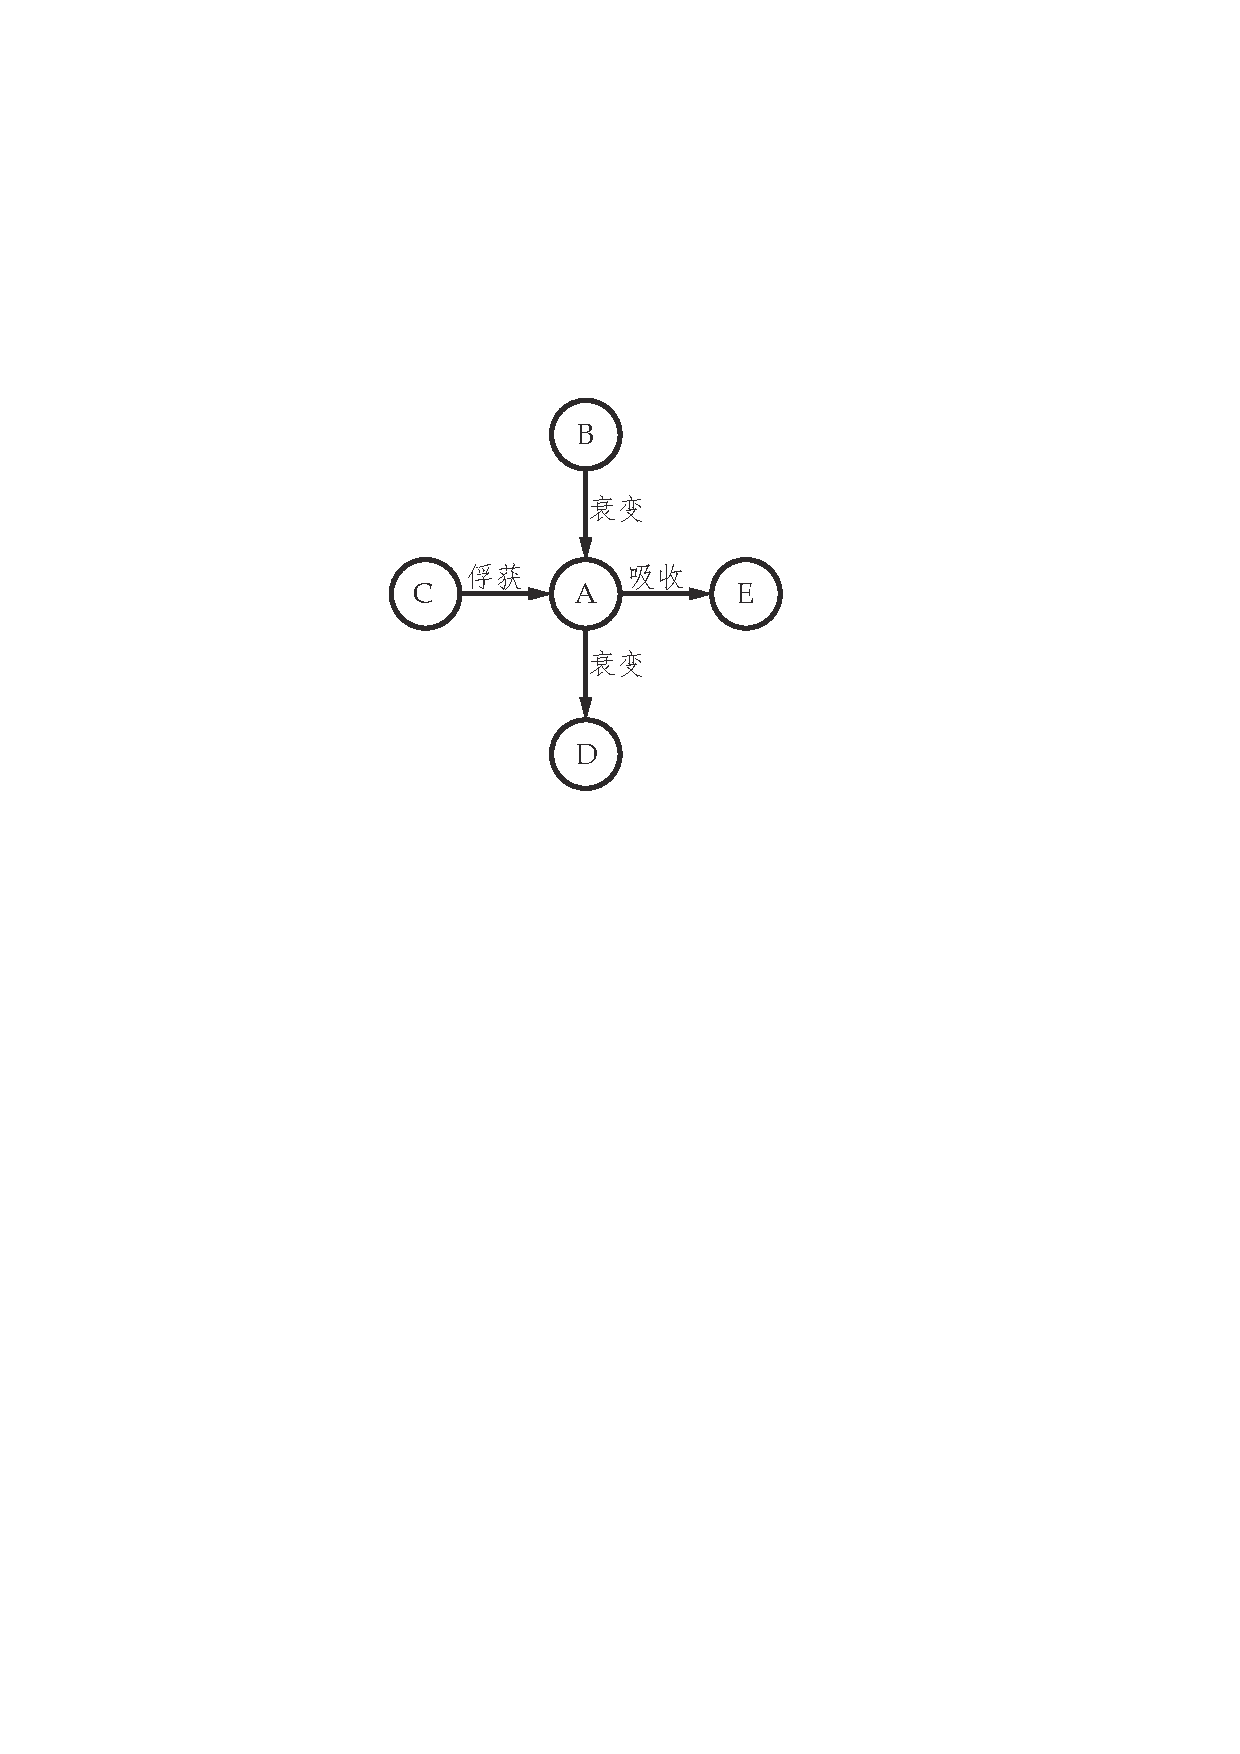
\includegraphics[scale=0.6]{figures/fig6.1.pdf}
            \end{minipage}
            \hfil
            \begin{minipage}{0.85\columnwidth}
                \begin{equation*}
                    \tikzmarknode{N}{\highlight{red}{$\dv{N_{\symrm{A}}(t)}{t}$}} =
                    \color{BlueViolet}
                    \overbrace{
                        \left(\tikzmarknode{C}{\highlight{Plum}{\color{black} $N_{\symrm{C}} \sigma_{\gamma,\,\symrm{C}} \phi$}} {\color{black} +} \tikzmarknode{B}{\highlight{NavyBlue}{\color{black}  $\lambda_{\symrm{B}} N_{\symrm{B}}$}}\right)
                    }^{\text{\fangsong \footnotesize \textcolor{BlueViolet!85}{核素A产生率}}}
                        \color{black} - 
                    \color{RawSienna}
                        \overbrace{
                        \left(\tikzmarknode{A1}{\highlight{Bittersweet}{\color{black} $N_{\symrm{A}} \sigma_{\symrm{a,\,A}} \phi$}} {\color{black} +} \tikzmarknode{A2}{\highlight{xkcdHunterGreen}{\color{black}   $\lambda_{\symrm{A}} N_{\symrm{A}}$}}\right)
                    }^{\text{\fangsong \footnotesize \textcolor{RawSienna!85}{核素A消失率}}}
                \end{equation*}
                \vspace*{0.5\baselineskip}
                \begin{tikzpicture}[overlay,remember picture,>=stealth,nodes={align=left,inner ysep=1pt},<-]
                    % 核素A变化率
                    \path (N.north) ++ (0,0.5em) node[anchor=south east,color=Maroon!85] (Ntext){\fangsong{\footnotesize 核素A变化率}};
                    \draw [color=Maroon](N.north) |- ([xshift=-0.3ex,color=Maroon]Ntext.south west);
                    % 核素C俘获中子产生A
                    \path (C.north) ++ (-3.2,-1.8em) node[anchor=north west,color=Plum!85] (Ctext){{\fangsong{\footnotesize 核素C俘获中子产生A}}};
                    \draw [color=Plum](C.south) |- ([xshift=-0.3ex,color=Plum]Ctext.south west);
                    % 核素B衰变产生A
                    \path (B.north) ++ (-2.6,-3.2em) node[anchor=north west,color=NavyBlue!85] (Btext){{\fangsong{\footnotesize 核素B衰变产生A}}};
                    \draw [color=NavyBlue](B.south) |- ([xshift=-0.3ex,color=NavyBlue]Btext.south west);
                    % 核素A吸收中子(裂变或俘获)消失
                    \path (A1.north) ++ (0.1,-3.2em) node[anchor=north west,color=Bittersweet!85] (A1text){\fangsong{\footnotesize 核素A吸收中子(裂变或俘获)消失}};
                    \draw [color=Bittersweet](A1.south) |- ([xshift=-0.3ex,color=Bittersweet]A1text.south east);
                    % 核素A衰变消失
                    \path (A2.north) ++ (0.1,-1.8em) node[anchor=north west,color=xkcdHunterGreen!85] (A2text){\fangsong{\footnotesize 核素A衰变消失}};
                    \draw [color=xkcdHunterGreen](A2.south) |- ([xshift=-0.3ex,color=xkcdHunterGreen]A2text.south east);
                \end{tikzpicture}
            \end{minipage}

            \vspace{1em}

            \item 假设a为中等质量核素或轻核素,\,有
            
            \vspace{1em}
            \begin{minipage}{0.1\columnwidth}
                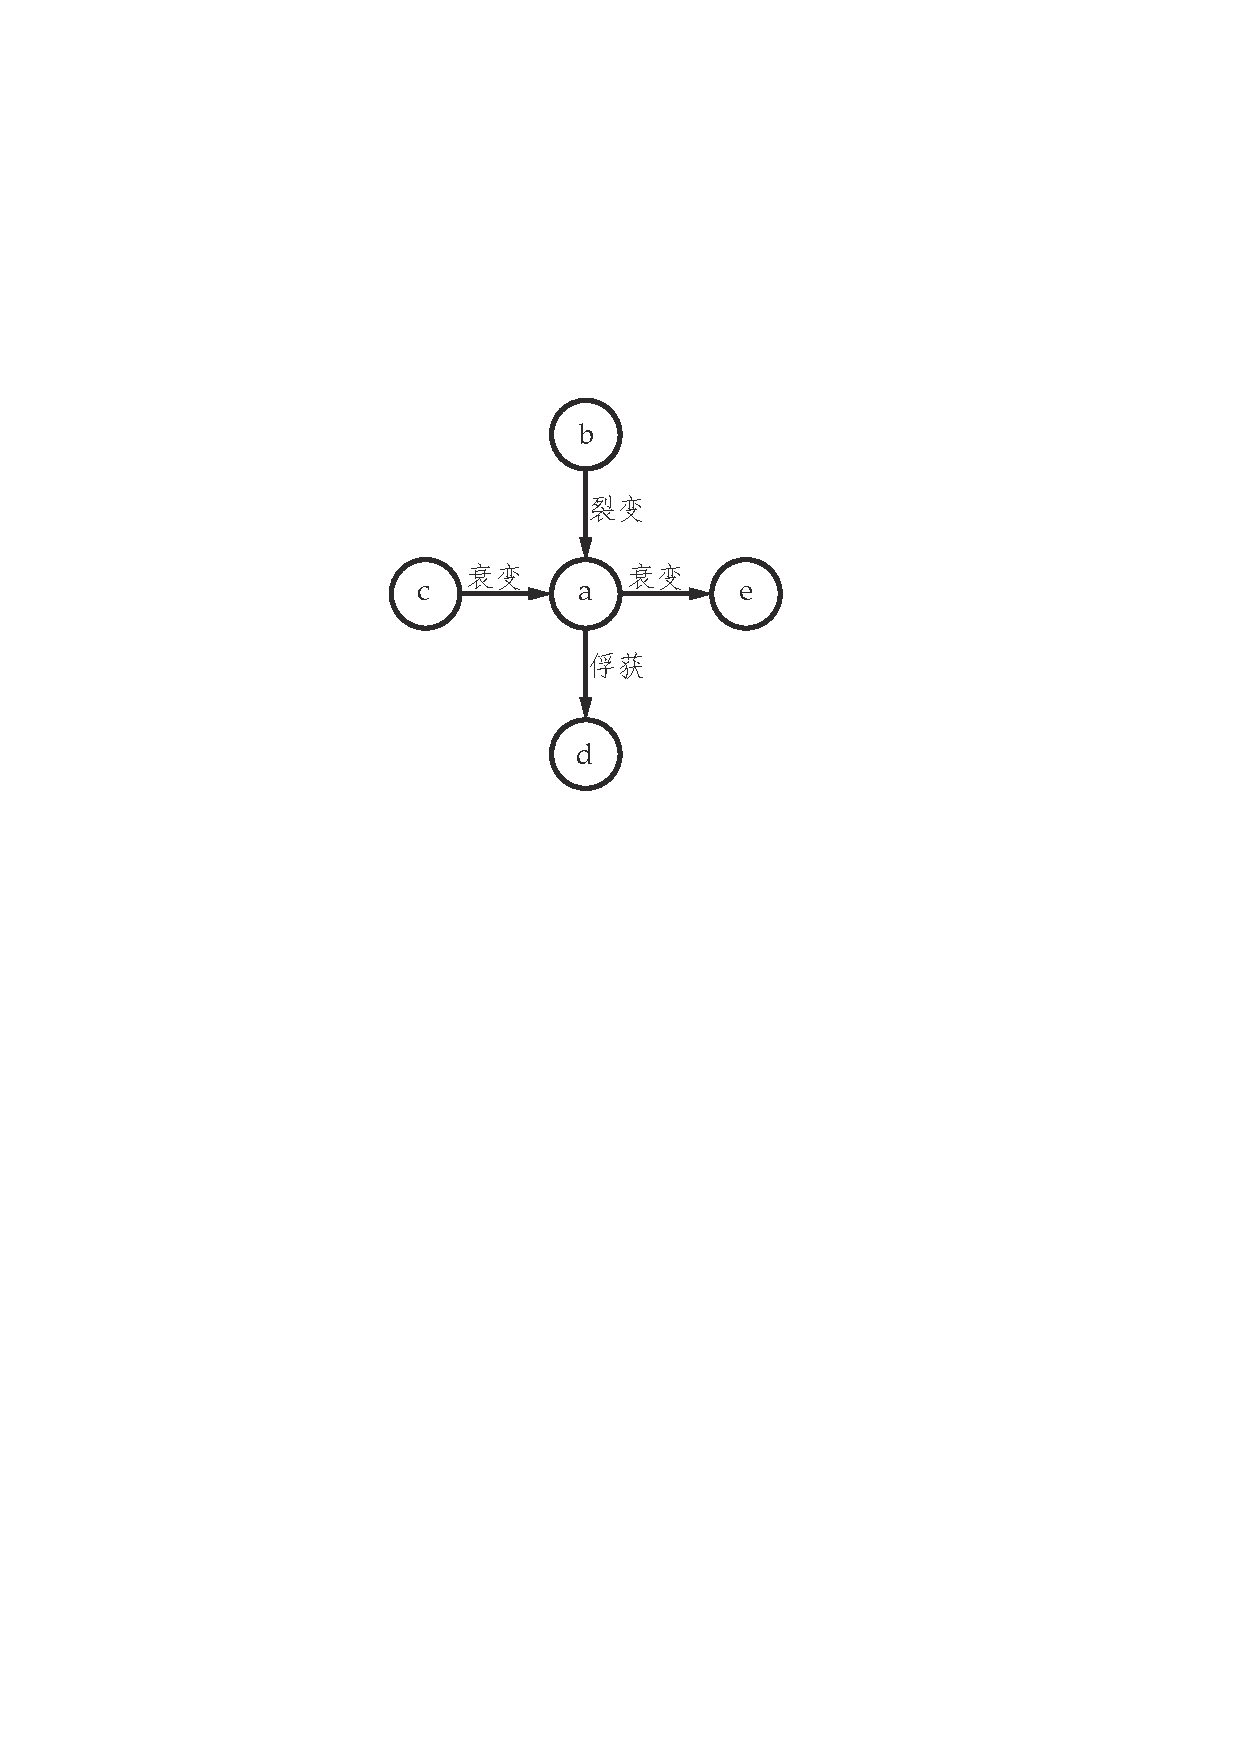
\includegraphics[scale=0.6]{figures/fig6.2.pdf}
            \end{minipage}
            \hfil
            \begin{minipage}{0.85\columnwidth}
                \begin{equation*}
                    \tikzmarknode{N}{\highlight{red}{$\dv{N_{\symrm{a}}(t)}{t}$}} =
                    \color{BlueViolet}
                    \overbrace{
                        \left(\tikzmarknode{C}{\highlight{Plum}{\color{black} $\gamma_{\symrm{a}} \vSigma_{\symrm{f}} \phi$}} {\color{black} +} \tikzmarknode{B}{\highlight{NavyBlue}{\color{black}  $\lambda_{\symrm{c}} N_{\symrm{c}}$}}\right)
                    }^{\text{\fangsong \footnotesize \textcolor{BlueViolet!85}{核素a产生率}}}
                        \color{black} - 
                    \color{RawSienna}
                        \overbrace{
                        \left(\tikzmarknode{A1}{\highlight{Bittersweet}{\color{black} $N_{\symrm{a}} \sigma_{\gamma,\,\symrm{a}} \phi$}} {\color{black} +} \tikzmarknode{A2}{\highlight{xkcdHunterGreen}{\color{black}   $\lambda_{\symrm{a}} N_{\symrm{a}}$}}\right)
                    }^{\text{\fangsong \footnotesize \textcolor{RawSienna!85}{核素a消失率}}}
                \end{equation*}
                \vspace*{0.5\baselineskip}
                \begin{tikzpicture}[overlay,remember picture,>=stealth,nodes={align=left,inner ysep=1pt},<-]
                    % 核素a变化率
                    \path (N.north) ++ (0,0.5em) node[anchor=south east,color=Maroon!85] (Ntext){\fangsong{\footnotesize 核素a变化率}};
                    \draw [color=Maroon](N.north) |- ([xshift=-0.3ex,color=Maroon]Ntext.south west);
                    % 核素b裂变产生a
                    \path (C.north) ++ (-3.2,-1.8em) node[anchor=north west,color=Plum!85] (Ctext){{\fangsong{\footnotesize 核素b裂变产生a}}};
                    \draw [color=Plum](C.south) |- ([xshift=-0.3ex,color=Plum]Ctext.south west);
                    % 核素c衰变产生a
                    \path (B.north) ++ (-2.6,-3.2em) node[anchor=north west,color=NavyBlue!85] (Btext){{\fangsong{\footnotesize 核素c衰变产生a}}};
                    \draw [color=NavyBlue](B.south) |- ([xshift=-0.3ex,color=NavyBlue]Btext.south west);
                    % 核素a俘获中子消失
                    \path (A1.north) ++ (0.1,-3.2em) node[anchor=north west,color=Bittersweet!85] (A1text){\fangsong{\footnotesize 核素a俘获中子消失}};
                    \draw [color=Bittersweet](A1.south) |- ([xshift=-0.3ex,color=Bittersweet]A1text.south east);
                    % 核素a衰变消失
                    \path (A2.north) ++ (0.1,-1.8em) node[anchor=north west,color=xkcdHunterGreen!85] (A2text){\fangsong{\footnotesize 核素a衰变消失}};
                    \draw [color=xkcdHunterGreen](A2.south) |- ([xshift=-0.3ex,color=xkcdHunterGreen]A2text.south east);
                \end{tikzpicture}
            \end{minipage}
        \end{enumerate}
    \end{solution}
\end{exercise}

\begin{exercise}
    试阐述什么是预估-校正法及其实现过程.\,
    \begin{solution}
        \begin{figure}[H]
            \centering
            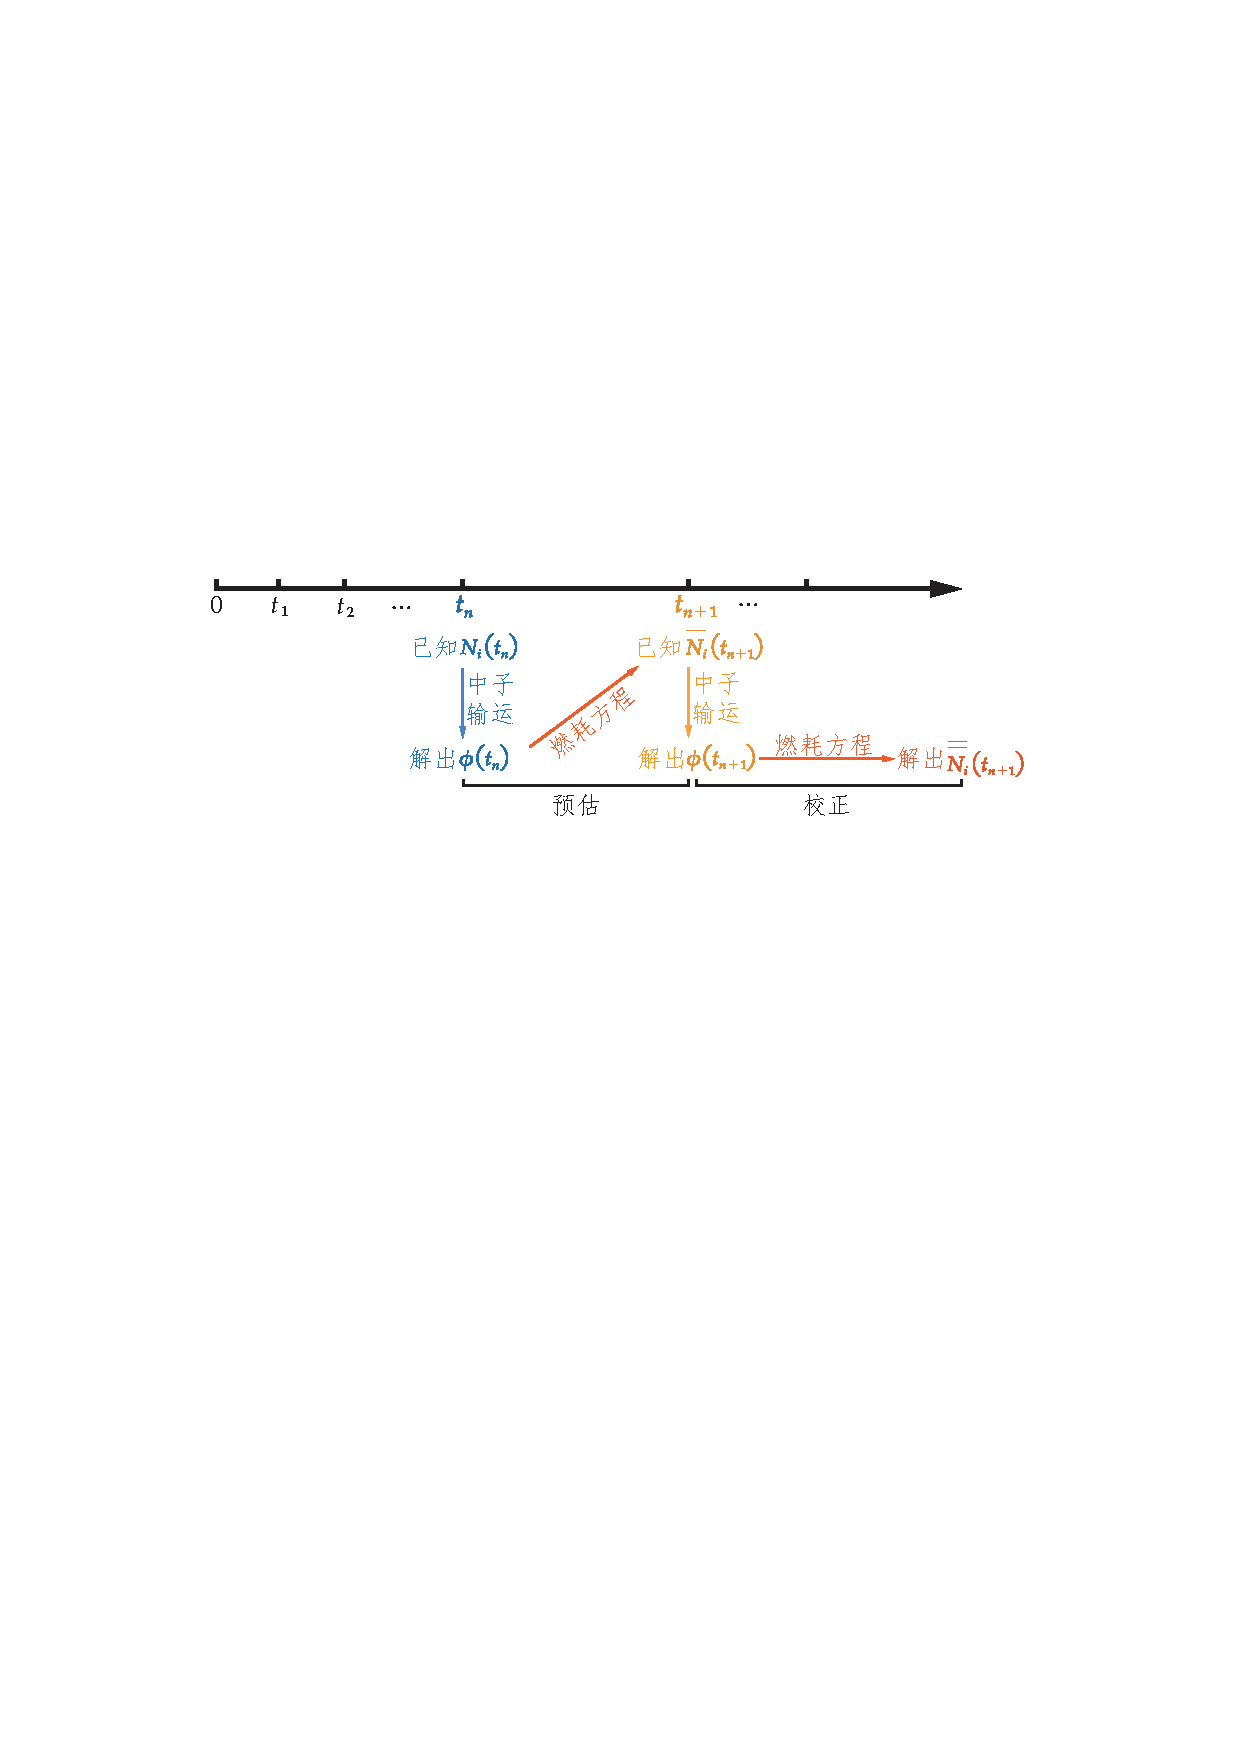
\includegraphics[scale=0.8]{figures/fig6.3.pdf}
        \end{figure}
    最后取
    \begin{equation*}
        N_i(t_{n+1}) = \frac{1}{2} \left[\overline{N_i}(t_{n+1}) + \overline{\overline{N_i}}(t_{n+1})\right]
    \end{equation*}
    \end{solution}
\end{exercise}

\begin{exercise}
    一座核反应堆,\,额定电功率为1200\,MW,\,热效率为30\%,\,每年平均更换1/3的燃料,\,在平衡状态下的平均卸料燃耗为15000\,MWd/tU,\,年平均负荷因子为0.8.\,试估算该核反应堆的铀装载量.\,(注:\,1年按照365天计)
    \begin{solution}
        核反应堆热功率
        \begin{equation*}
            P_{\symrm{h}} = \frac{P_{\symrm{e}}\eta}{\eta_{\symrm{e}}} = \frac{1200 \times 0.8}{0.3}\,\symrm{MW} = 3200\,\symrm{MW}
        \end{equation*}
        铀装载量
        \begin{equation*}
            m_{\symrm{U}} = \frac{P_{\symrm{h}} \times 365}{15000} \times 3 = \frac{3200 \times 365}{15000} \times 3\,\symrm{tU} = 233.6\,\symrm{tU}
        \end{equation*}
    \end{solution}
\end{exercise}

\begin{exercise}
    在一座功率运行的核反应堆中,\,${}^{135}\symrm{Xe}$的产生主要是来自\underline{{\kaishu ${}^{135}\symrm{I}$衰变}},\,其次是来自\underline{{\kaishu ${}^{235}\symrm{U}$裂变}}.\,
\end{exercise}

\begin{exercise}
    一座满功率运行的压水堆突然停堆,\,试画出${}^{135}\symrm{I},\,{}^{135}\symrm{Xe}$的原子核密度和剩余反应性$\rho_{\symrm{ex}}$随时间的变化曲线,\,并在图中标出碘坑时间$t_{\symrm{I}}$,\,强迫停堆时间$t_{\symrm{f}}$,\,允许停堆时间$t_{\symrm{p}}$,\,最大碘坑时间$t_{\symrm{max}}$,\,以及碘坑深度$\Delta\rho_{\symrm{ex,\,I}}$.\,
    \begin{solution}
        \begin{figure}[H]
            \centering
            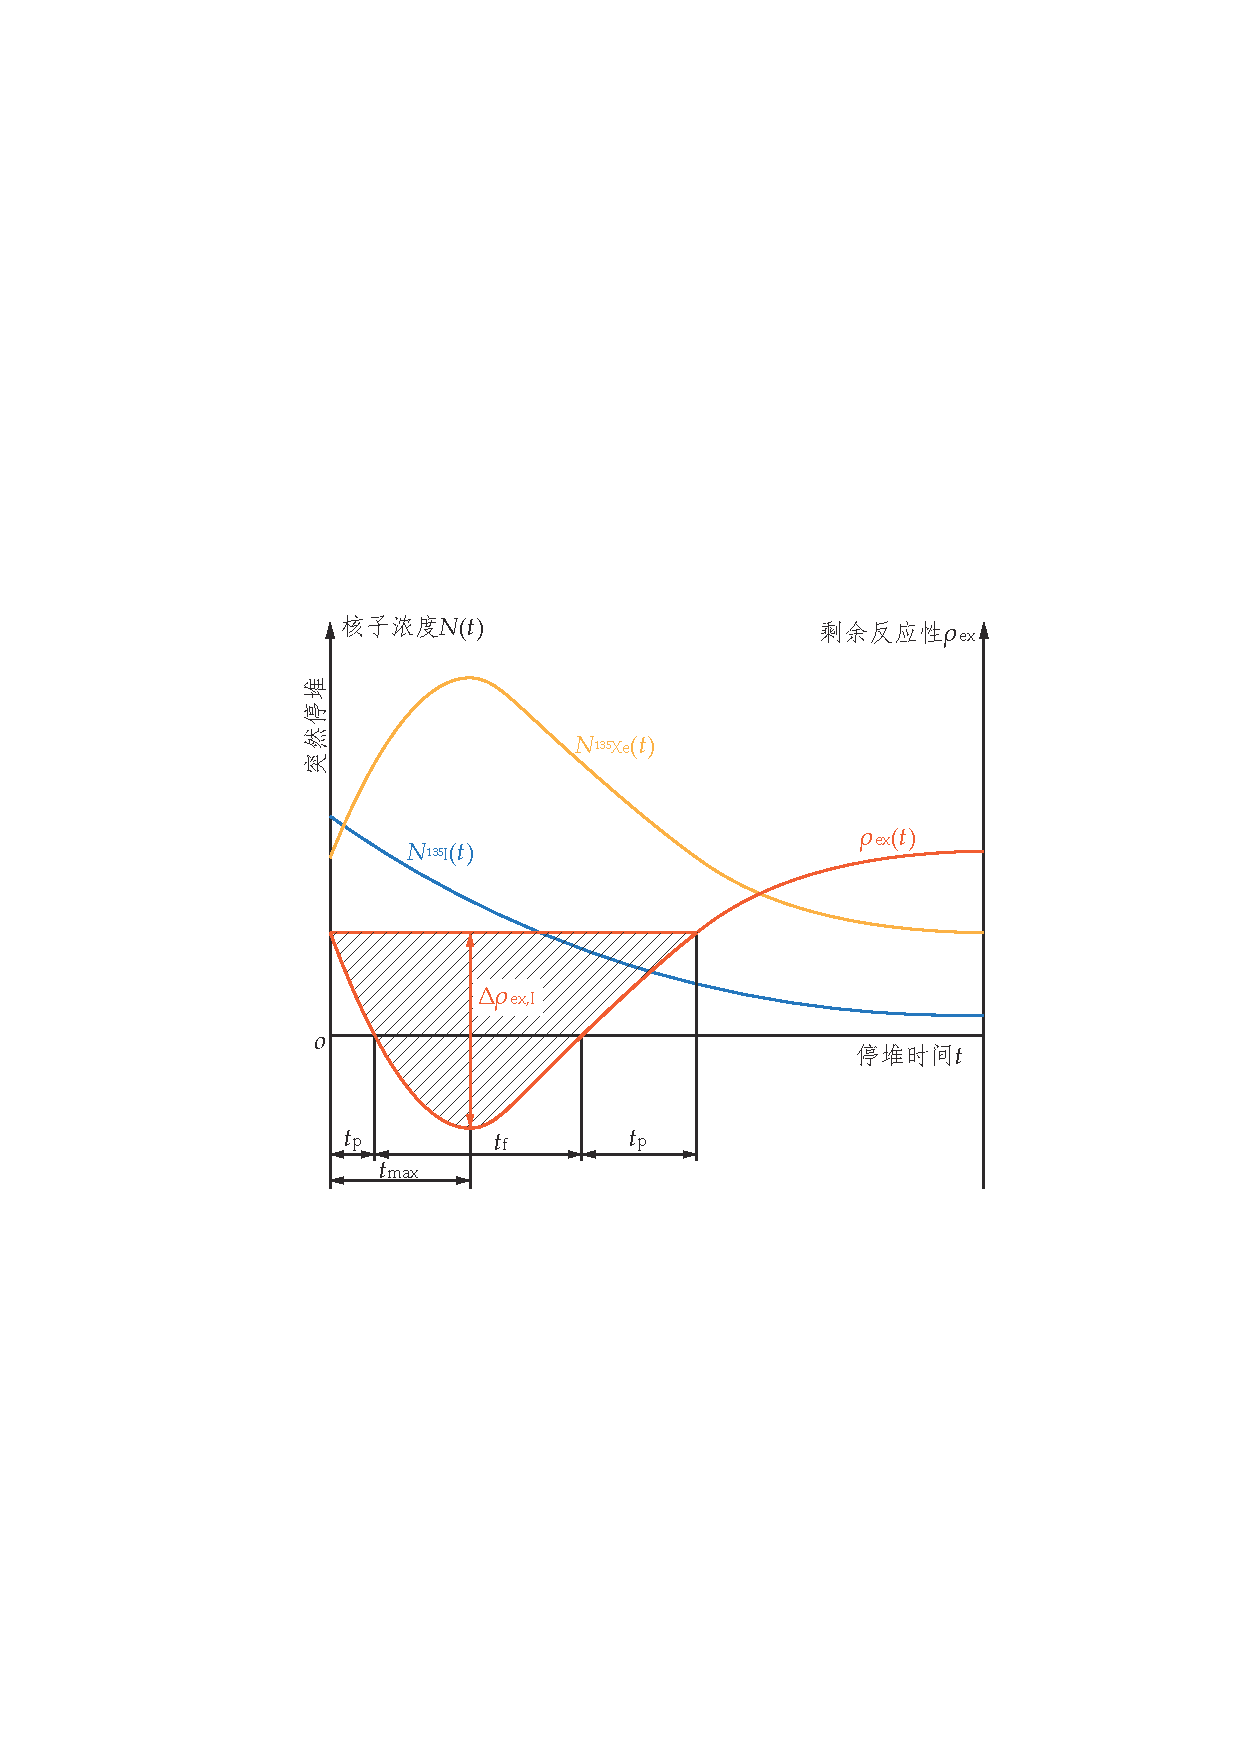
\includegraphics[scale=0.9]{figures/fig6.4.pdf}
        \end{figure}
    \end{solution}
\end{exercise}

\begin{exercise}
    一座压水堆,\,先以满功率运行200天,\,然后一次性将功率降至50\%FP,\,并稳定运行. 
    \begin{enumerate}[(1)]
        \item 试画出该过程中${}^{135}\symrm{I}$和${}^{135}\symrm{Xe}$的原子核密度随时间的变化曲线;
        \item 试画出该过程中${}^{149}\symrm{Pm}$和${}^{149}\symrm{Sm}$的原子核密度随时间的变化曲线.
    \end{enumerate}
    \begin{solution}
        \begin{enumerate}[(1)]
            \item 碘-氙
            \begin{figure}[H]
                \centering
                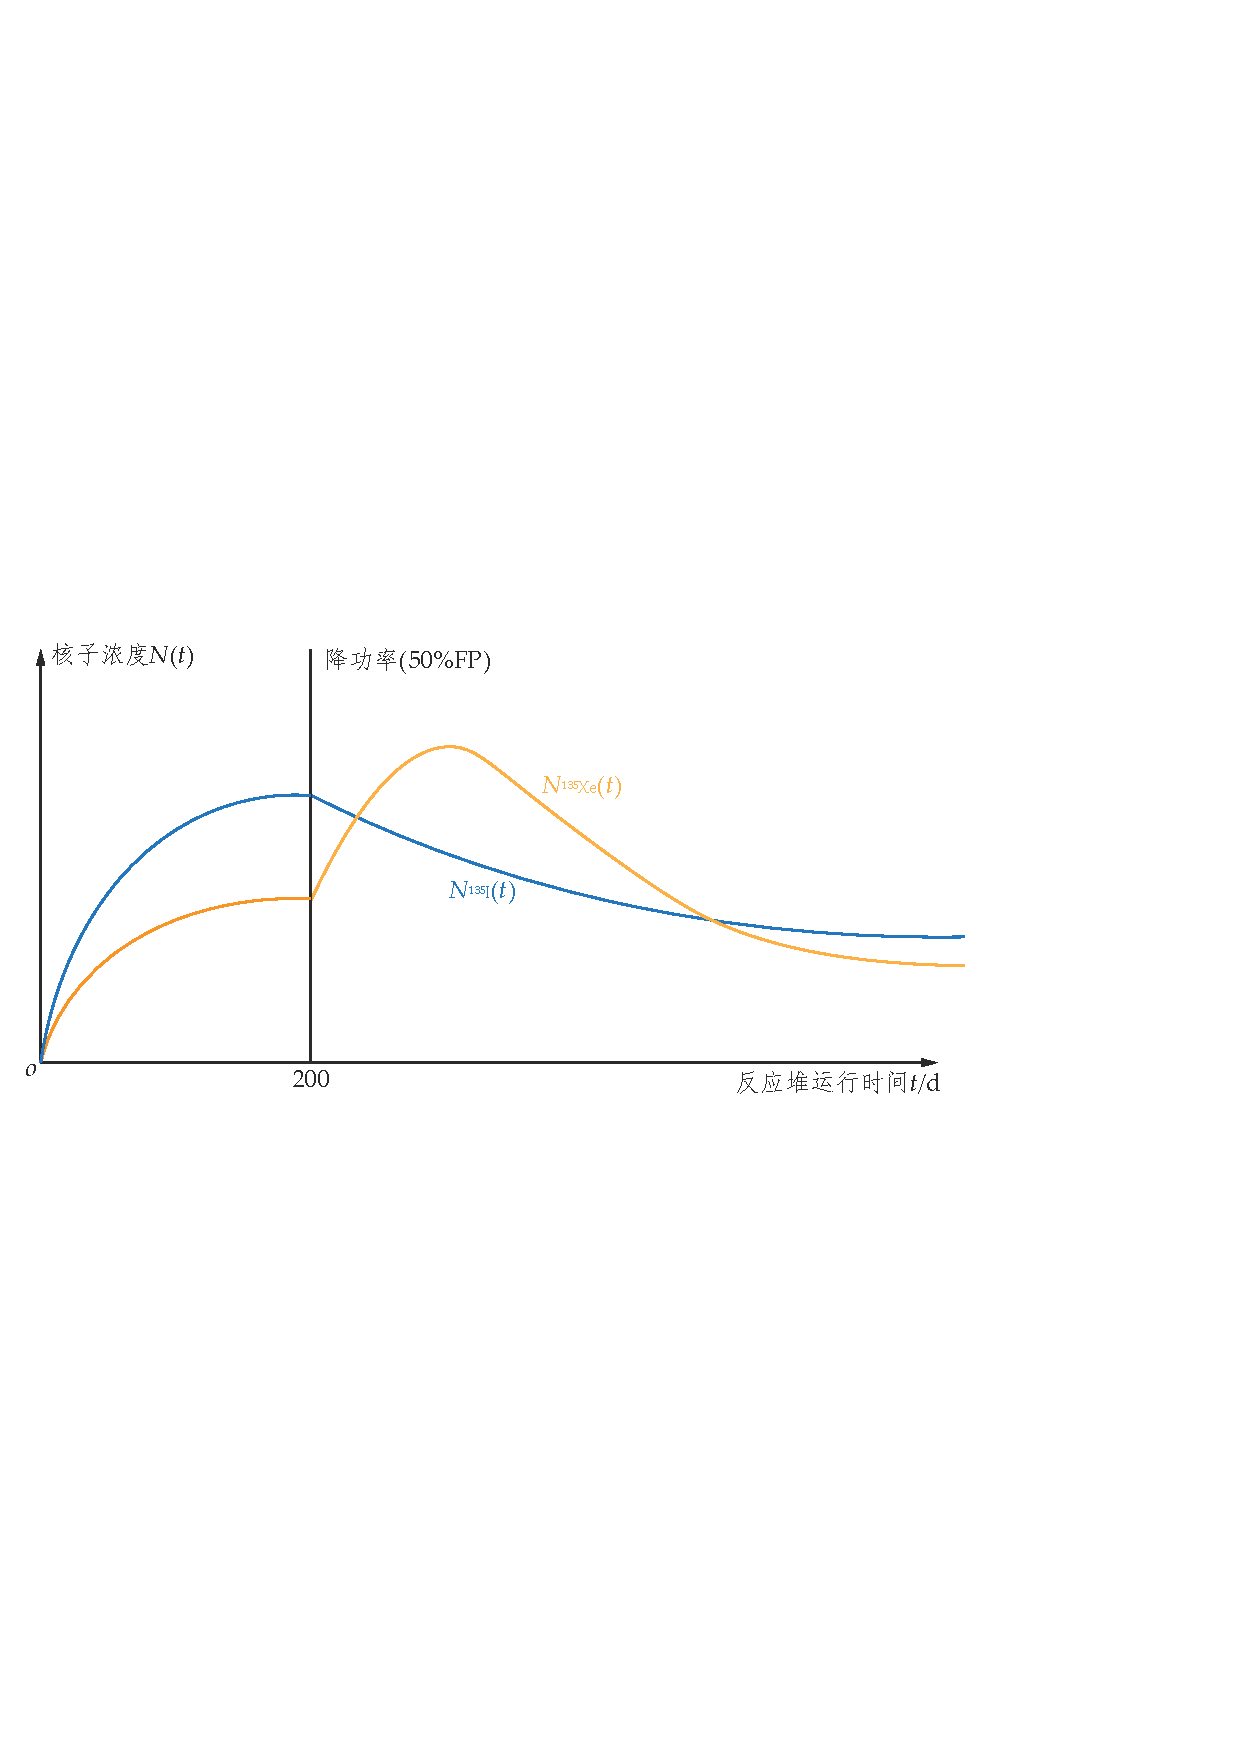
\includegraphics[scale=0.75]{figures/fig6.5.pdf}
            \end{figure}
            \item 钷-钐
            \begin{figure}[H]
                \centering
                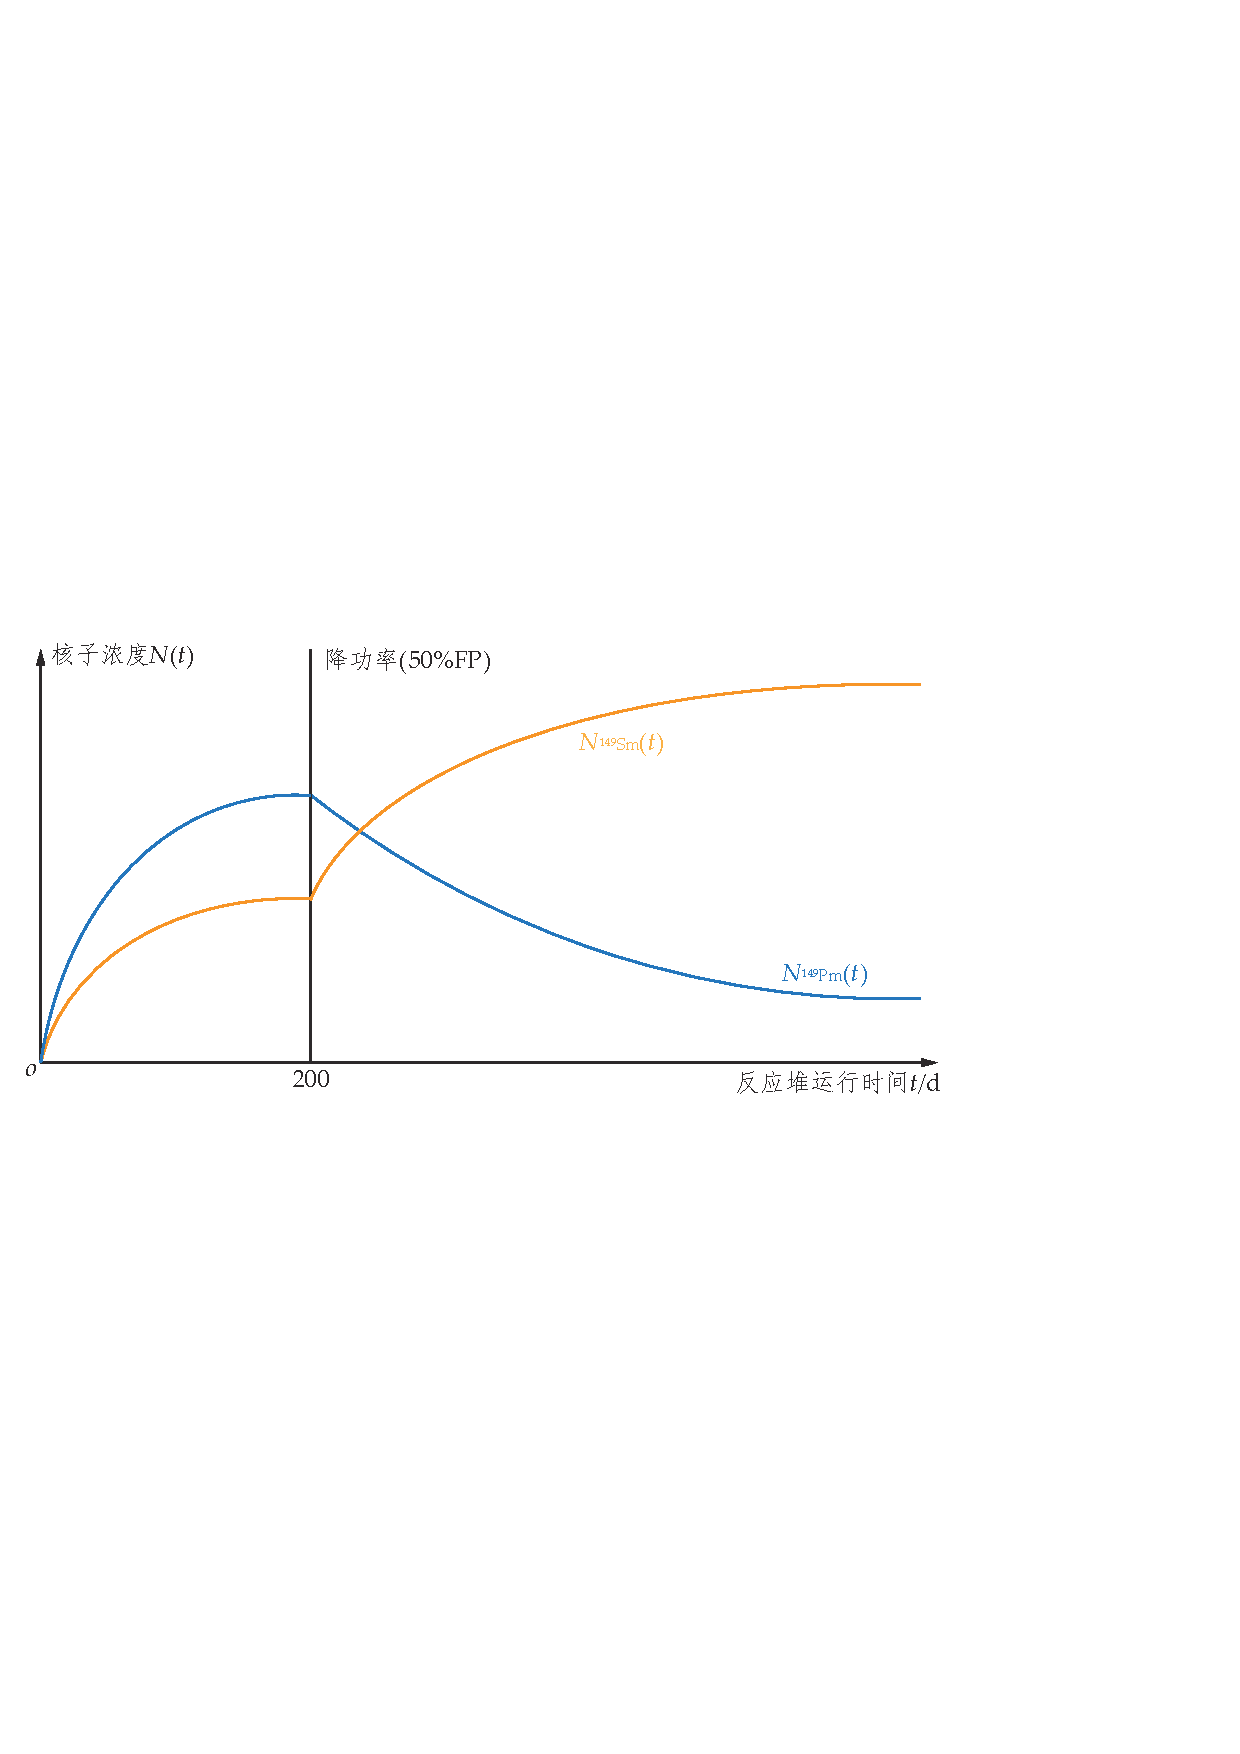
\includegraphics[scale=0.75]{figures/fig6.6.pdf}
            \end{figure}
        \end{enumerate}
    \end{solution}
\end{exercise}

\begin{exercise}
    试画出碘-氙衰变链,\,并根据平衡关系写出压水堆运行中碘和氙的原子核密度变化关系以及碘、氙的平衡浓度.\,
    \begin{solution}

        \begin{minipage}{0.2\columnwidth}
            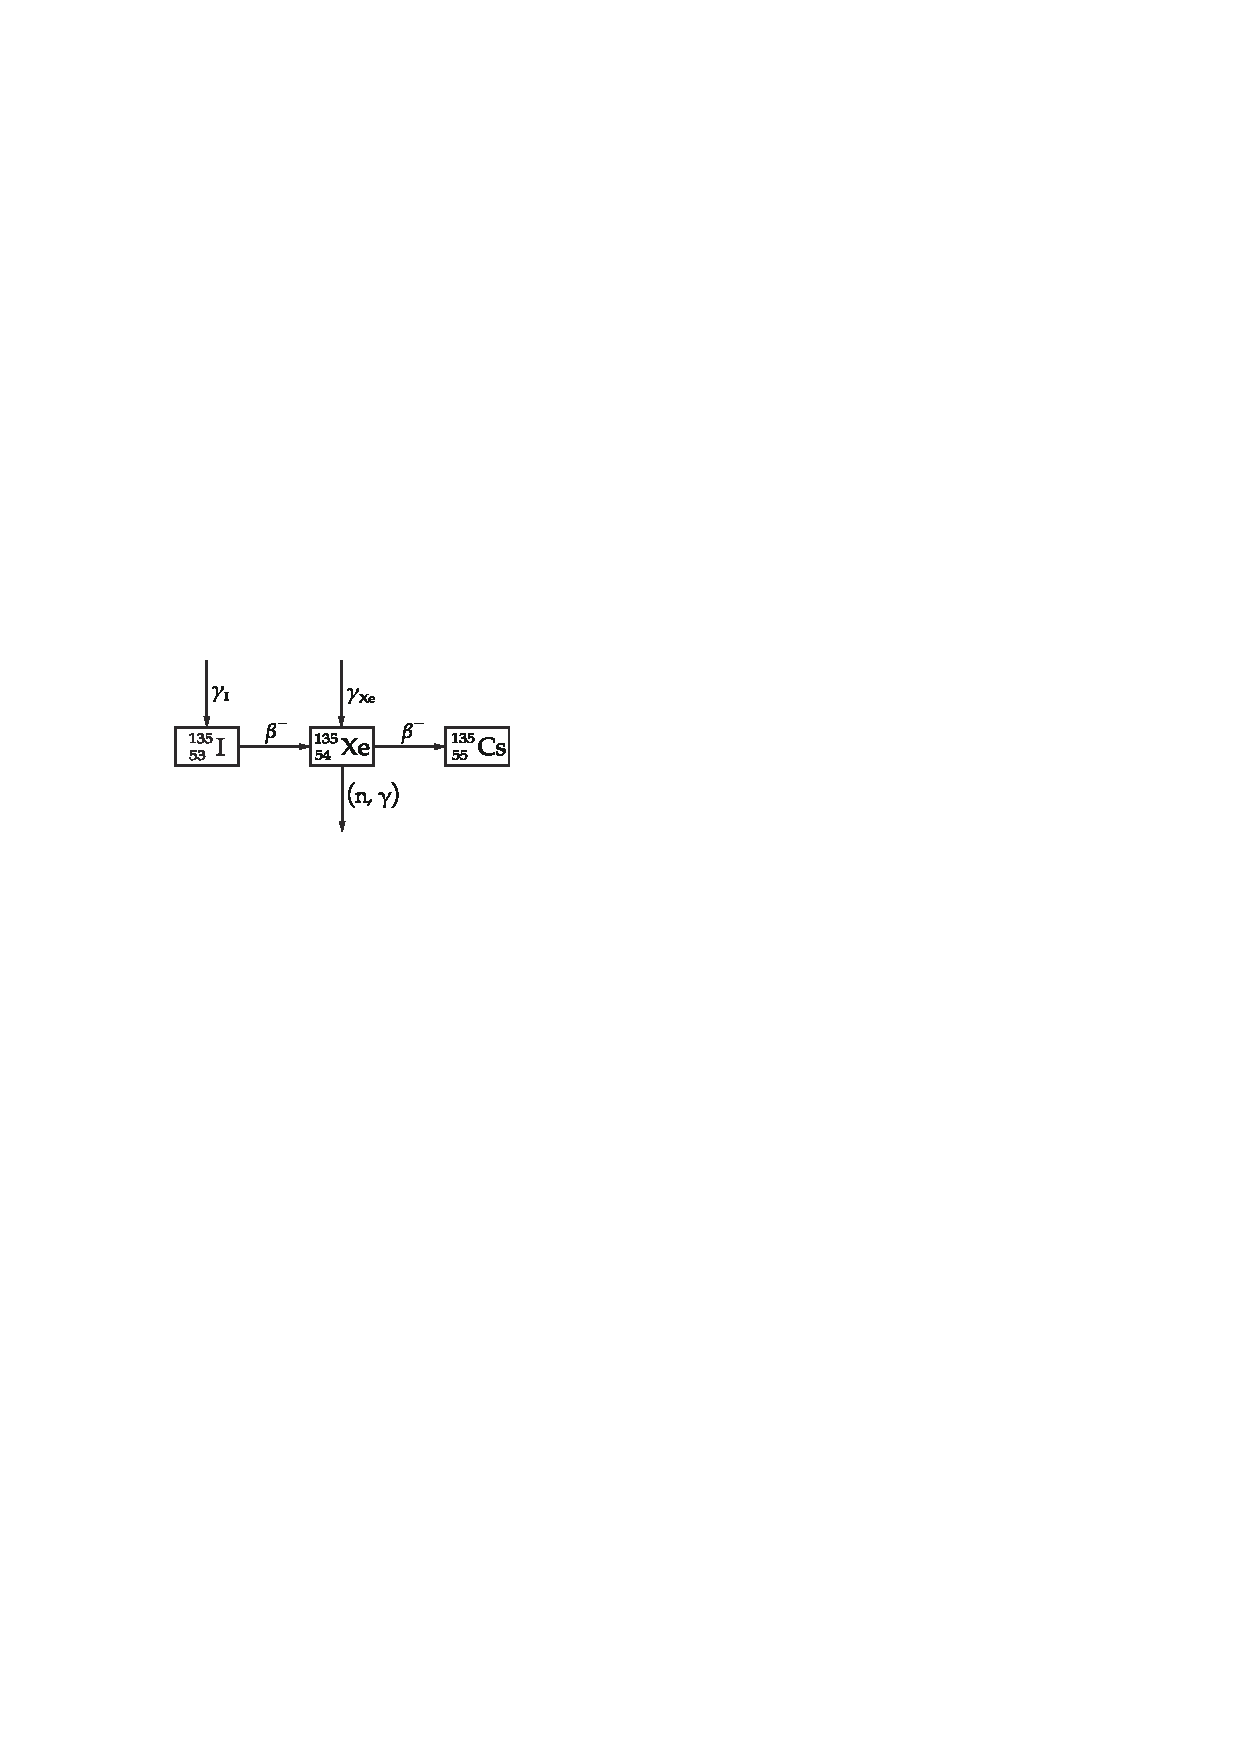
\includegraphics[scale=0.8]{figures/fig6.7.pdf}
        \end{minipage}
        \hfil
        \begin{minipage}{0.8\columnwidth}
            \begin{align*}
                & \dv{N_{\symrm{I}}(t)}{t} = \gamma_{\symrm{I}} \vSigma_{\symrm{f}} \phi - \lambda_{\symrm{I}} N_{\symrm{I}}(t) \\
                & \dv{N_{\symrm{Xe}}(t)}{t} = \gamma_{\symrm{Xe}} \vSigma_{\symrm{f}} \phi + \lambda_{\symrm{I}} N_{\symrm{I}}(t) - \left(\lambda_{\symrm{Xe}} + \sigma_{\gamma}^{\symrm{Xe}} \phi\right) N_{\symrm{Xe}}(t)
            \end{align*}
        \end{minipage}

        当$t \to \infty$,\,碘和氙达到平衡浓度时,\,$\dv{N_i(t)}{t} = 0$,\,于是
        \begin{align*}
            & N_{\symrm{I}}(\infty) = \frac{\gamma_{\symrm{I}} \vSigma_{\symrm{f}} \phi}{\lambda_{\symrm{I}}} \\
            & N_{\symrm{Xe}}(\infty) = \frac{(\gamma_{\symrm{I}} + \gamma_{\symrm{Xe}}) \vSigma_{\symrm{f}} \phi}{\lambda_{\symrm{Xe}} + \sigma_{\gamma}^{\symrm{Xe}}}
        \end{align*}
    \end{solution}
\end{exercise}

\begin{exercise}
    试画出钜-钐衰变链,\,并根据平衡关系写出压水堆运行中饱和钐的原子核密度变化关系以及钜和钐的平衡浓度.\,
    \begin{solution}

        \begin{minipage}{0.1\columnwidth}
            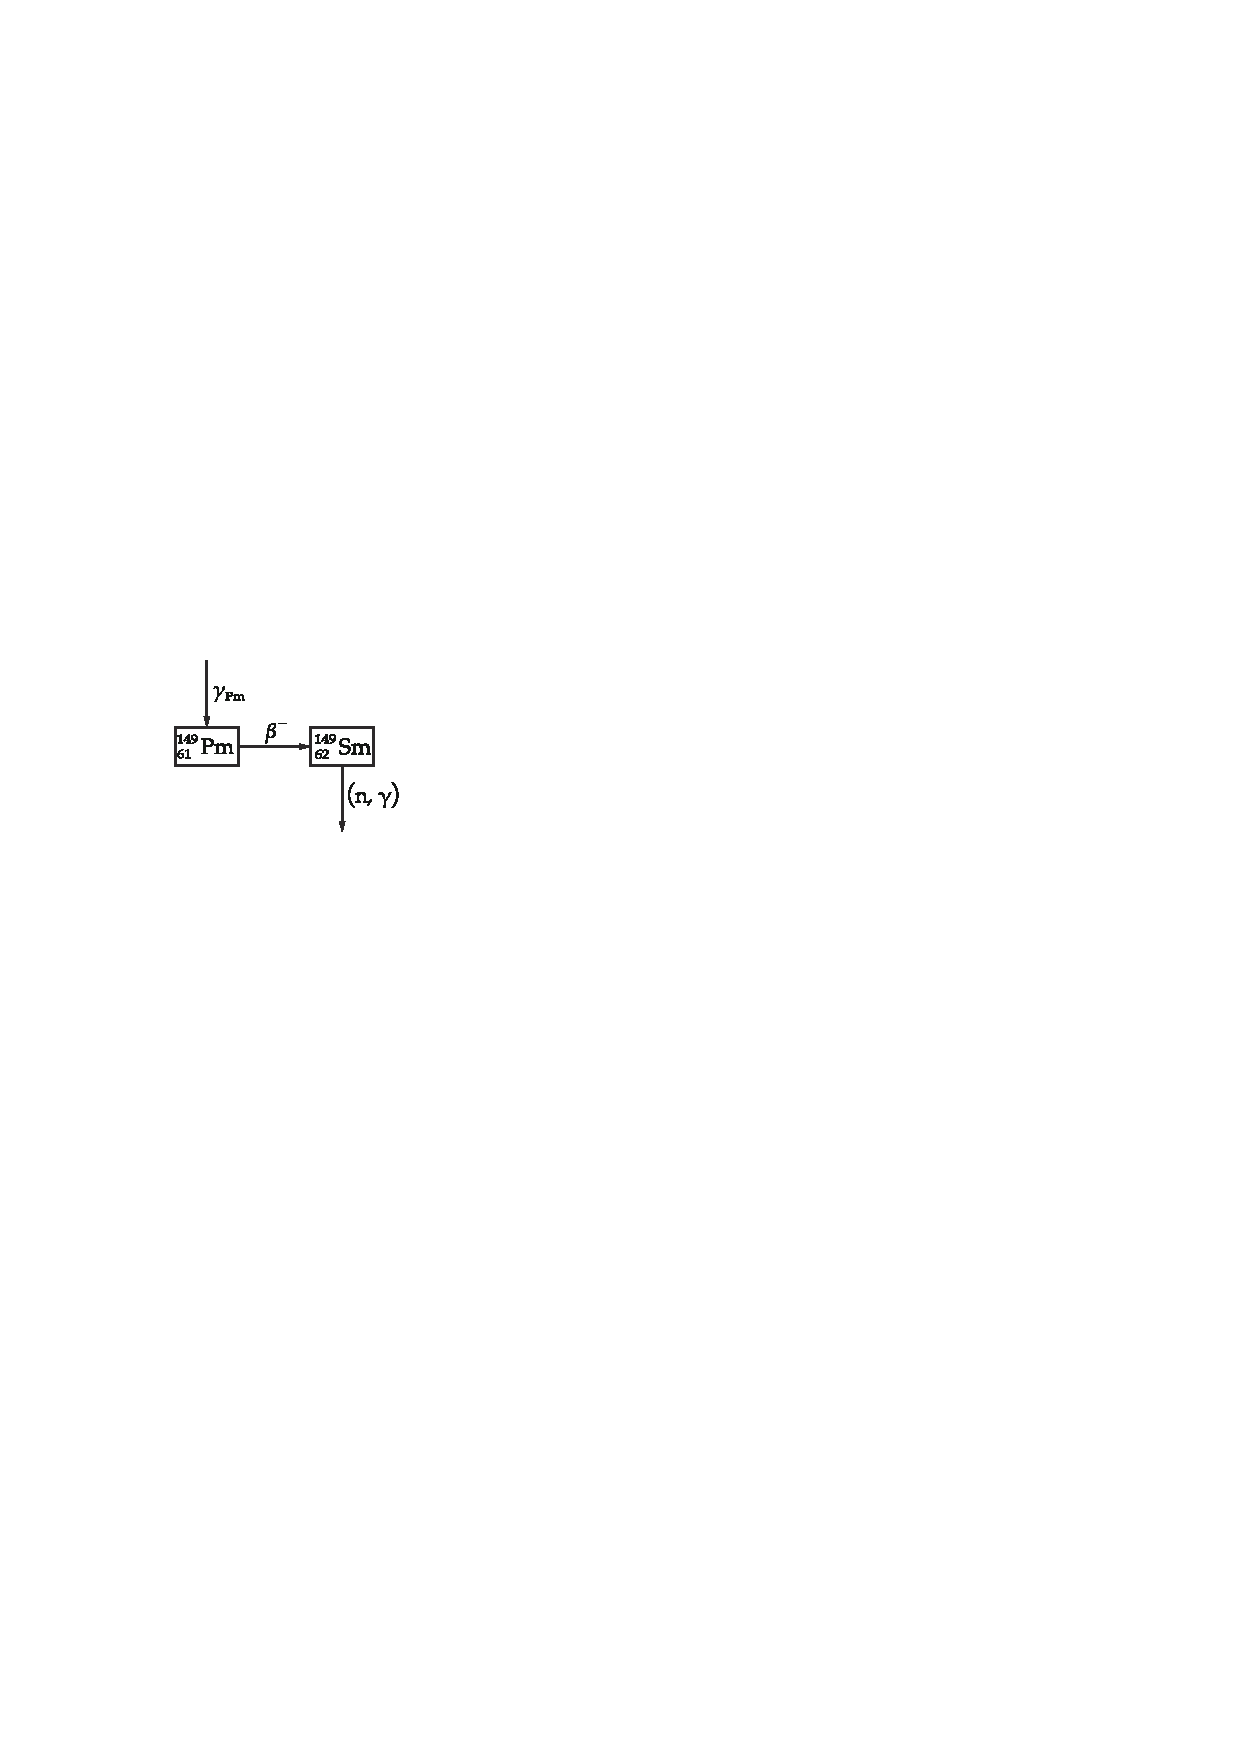
\includegraphics[scale=0.9]{figures/fig6.8.pdf}
        \end{minipage}
        \hfil
        \begin{minipage}{0.9\columnwidth}
            \begin{align*}
                & \dv{N_{\symrm{Pm}}(t)}{t} = \gamma_{\symrm{Pm}} \vSigma_{\symrm{f}} \phi - \lambda_{\symrm{Pm}} N_{\symrm{Pm}}(t) \\
                & \dv{N_{\symrm{Sm}}(t)}{t} = \lambda_{\symrm{Pm}} N_{\symrm{Pm}}(t) - \sigma_{\gamma}^{\symrm{Sm}} \phi N_{\symrm{Sm}}(t)
            \end{align*}
        \end{minipage}

        当$t \to \infty$,\,钷和钐达到平衡浓度时,\,$\dv{N_i(t)}{t} = 0$,\,于是
        \begin{align*}
            & N_{\symrm{Pm}}(\infty) = \frac{\gamma_{\symrm{Pm}} \vSigma_{\symrm{f}} \phi}{\lambda_{\symrm{Pm}}} \\
            & N_{\symrm{Sm}}(\infty) = \frac{\gamma_{\symrm{Pm}} \vSigma_{\symrm{f}}}{\sigma_{\gamma}^{\symrm{Sm}}}
        \end{align*}
    \end{solution}
\end{exercise}

\begin{exercise}
    一座热中子核反应堆,\,在低功率水平下运行到第42周时发生了紧急停堆,\,在12个小时后恢复临界,\,然后以一定的速率在6小时内将功率提升到60\%FP.\,为了在该水平下达到氙平衡状态,\,需要多长时间?\,\xparen
    \begin{xchoices}[showanswer=true]
        \item 20到30个小时
        \item* 40到50个小时
        \item 70到80个小时
        \item 不知道先前的功率运行史,\,不能确定需要多长时间
    \end{xchoices}
    \vspace{1em}
\end{exercise}

\begin{exercise}
    产生氙振荡的条件有哪些?\,
    \begin{solution}
        \begin{enumerate}[(1)]
            \item 核反应堆属于热中子反应堆;
            \item 核反应堆足够大.
        \end{enumerate}
    \end{solution}
\end{exercise}